\documentclass[11pt]{article}
\usepackage[utf8]{inputenc}
\usepackage{float}
\usepackage{amsmath}
\usepackage{tikz} % for Hasse diagram
\usepackage[hmargin=3cm,vmargin=6.0cm]{geometry}
%\topmargin=0cm
\topmargin=-2cm
\addtolength{\textheight}{6.5cm}
\addtolength{\textwidth}{2.0cm}
%\setlength{\leftmargin}{-5cm}
\setlength{\oddsidemargin}{0.0cm}
\setlength{\evensidemargin}{0.0cm}

\begin{document}
	
\section*{Student Information } 
%Write your full name and id number between the colon and newline
%Put one empty space character after colon and before newline
Full Name : Ertuğrul Aypek  \\
Id Number : 2171270 \\

% Write your answers below the section tags
\section*{Answer 1}
Let a denote number of vertices: \\
It is said that all vertices have at least degree 4, so there is at least 4a/2 = 2a edges in our graph. \\
And number of edges is given 23. \\
So, 2a$<$23 \\
a$<$11,5 \\
Hence we can have maximum 11 vertices in our graph.

\section*{Answer 2}


\section*{Answer 3}


\section*{Answer 4}
\begin{itemize}
	\item[\textbf{a.}]
	\begin{tabular}{•}
	
	\end{tabular}
	
	
	 
	\item[\textbf{b.}] 
\end{itemize}

\begin{figure}[H]	\caption{Delete the related edges to display the acquired MST}
	\centering
	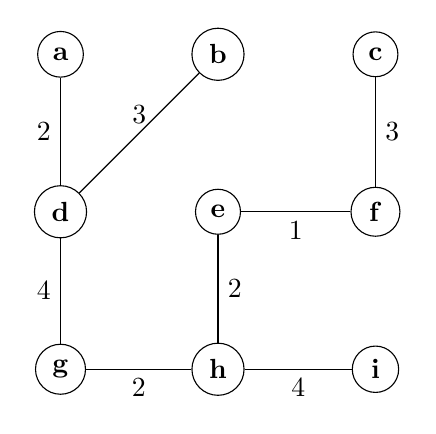
\begin{tikzpicture}
	
	\node[shape=circle,draw=black] (a) at (0, 4)     {\textbf{a}};
	\node[shape=circle,draw=black] (b) at (2, 4)     {\textbf{b}};
	\node[shape=circle,draw=black] (c) at (4, 4)     {\textbf{c}};
	\node[shape=circle,draw=black] (d) at (0, 2)     {\textbf{d}};
	\node[shape=circle,draw=black] (e) at (2, 2)     {\textbf{e}};
	\node[shape=circle,draw=black] (f) at (4, 2)     {\textbf{f}};
	\node[shape=circle,draw=black] (g) at (0, 0)     {\textbf{g}};
	\node[shape=circle,draw=black] (h) at (2, 0)     {\textbf{h}};
	\node[shape=circle,draw=black] (i) at (4, 0)     {\textbf{i}};
	
	
	\path[-] (a) edge  node[left]  {2} (d);
	\path[-] (b) edge  node[above] {3} (d);
	
	
	
	\path[-] (c) edge  node[right] {3} (f);
	

	\path[-] (d) edge  node[left]  {4} (g);
	\path[-] (e) edge  node[right] {2} (h);
	\path[-] (e) edge  node[below] {1} (f);
	
	
	\path[-] (g) edge  node[below] {2} (h);
	\path[-] (h) edge  node[below] {4} (i);
	
	\end{tikzpicture} 
\end{figure}

\end{document}